
\documentclass[9pt,twocolumn,twoside,lineno]{gsajnl}
\usepackage{epstopdf}
\usepackage[utf8]{vietnam}
\articletype{inv} 
\graphicspath{ {Figs/} } 

\runningtitle{Assignment 2 - Group 9} 
\runningauthor{FOBE}

\title{Computer Networks and the Internet - \textit{Assignment 2}}

\author[1,$\dagger$]{Nguyen Hoang Tan}
\author[2]{Le Thi Kim Yen}
\author[3]{Pham Tram Anh}
\author[4]{Le Gia Khang}


\affil[1]{Write report}
\affil[2]{Question 1}
\affil[3]{Question 2}
\affil[4]{Question 3}
\affil[$\dagger$]{These authors contributed equally to this work.}




\begin{abstract}
Thông qua việc trả lời 3 câu hỏi trong \textit{Assignment 2} chúng ta sẽ tìm hiểu về 2 vấn đề chính. Như đã học ở phần trước, có
2 phương thức chuyển mạch chính được sử dụng hiện nay là \textit{Chuyển mạch gói} và \textit{Chuyển mạch kênh}, bài này sẽ phân tích sự
khác nhau giữa chúng. Ngoài ra ta còn tìm hiểu vì sao phải chia mạng Internet thành nhiều tầng khác nhau và chức năng chính của mỗi tầng là gì. 
\end{abstract}

\keywords{Circuit switching; Packet Switching; OSI}



\begin{document}
\maketitle
\thispagestyle{firststyle}

\vspace{-13pt}



\section{Điểm chung giữa chuyển mạch gói và chuyển mạch kênh}

Đều là phương pháp truyền thông tin, dữ liệu thuộc tầng Application thông qua thiết bị đầu cuối và các nút mạng. Các thông tin, dữ liệu được truyền tải thông qua các đường link

\section{Sự khác biệt giữa 2 phương pháp}
\subsection{Chuyển mạch gói}
Host chia nhỏ aplication - layer messages thành các packets. Chuyển tiếp các gói từ một bộ định tuyến này đến bộ định
tuyến tiếp theo qua các đường link trên đường đi từ nguồn đến đích.


\begin{figure}[h]
  \centering
  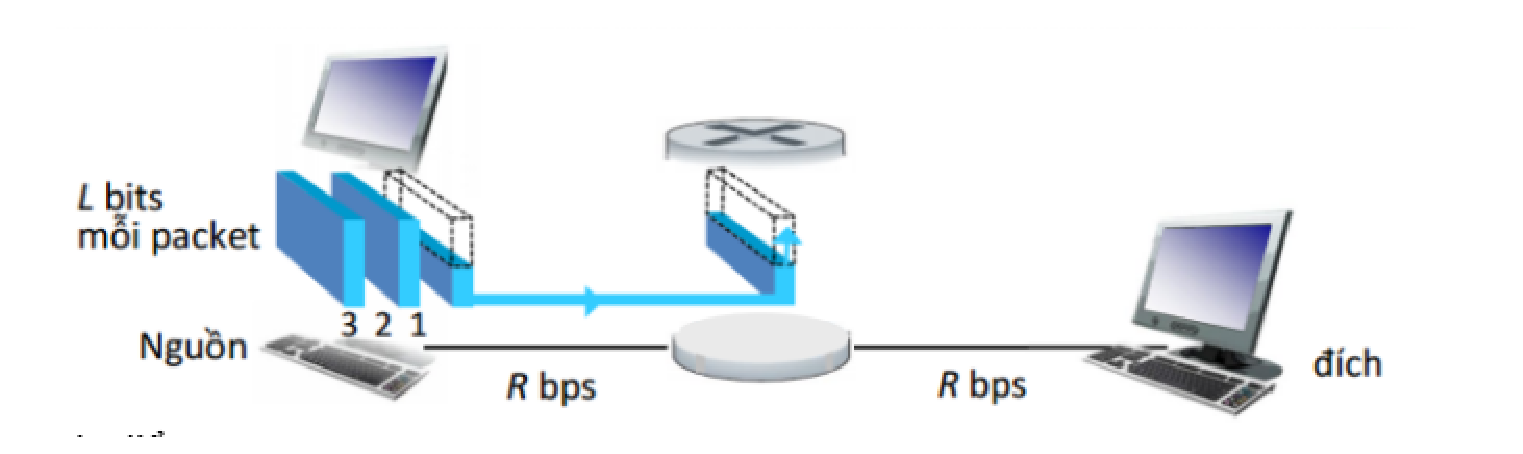
\includegraphics[scale=0.3]{q1_1}
  \caption{Hosts chia nhỏ application và chuyển nó theo qua các đường link.}
  \label{fig:my_label}
\end{figure}

\subsubsection{Ưu điểm}
\begin{itemize}
  \item Mỗi packet được truyền tải với công suất lớn nhất của đường link;
  \item Nhiều người được sử dụng mạng vì các đường link không bị chiếm giữ liên tục;
  \item Hiệu suất cao vì kích thước các gói tin được thiết kế sao cho nút mạng có thể xử lí nhanh nhất mà không
  cần lưu trữ tạm thời trên đĩa;
\end{itemize}
\subsubsection{Nhược điểm\\}
Vấn đề khó khăn nhất của mạng loại này là việc tập hợp các gói tin để tạo thành bản thông báo ban đầu của người sử dụng, đặc biệt trong trường hợp các gói được truyền theo nhiều đường khác nhau.
Cần phải đặt các cơ chế “đánh dấu” gói tin và phục hồi các gói tin bị thất lạc nếu xãy ra lỗi giữa các nút mạng. \\
Xếp hàng và sự mất mát: Nếu tốc độ đến (theo bit) đến đường link vượt qua tốc độ truyền dẫn của đường link trong một khoảng thời gian:\\

\begin{itemize}
  \item Các packet sẽ xếp hàng và đợi để được truyền tải trên đường link làm tốc độ truyền tải bị hạn chế;
  \begin{figure}[h]
    \centering
    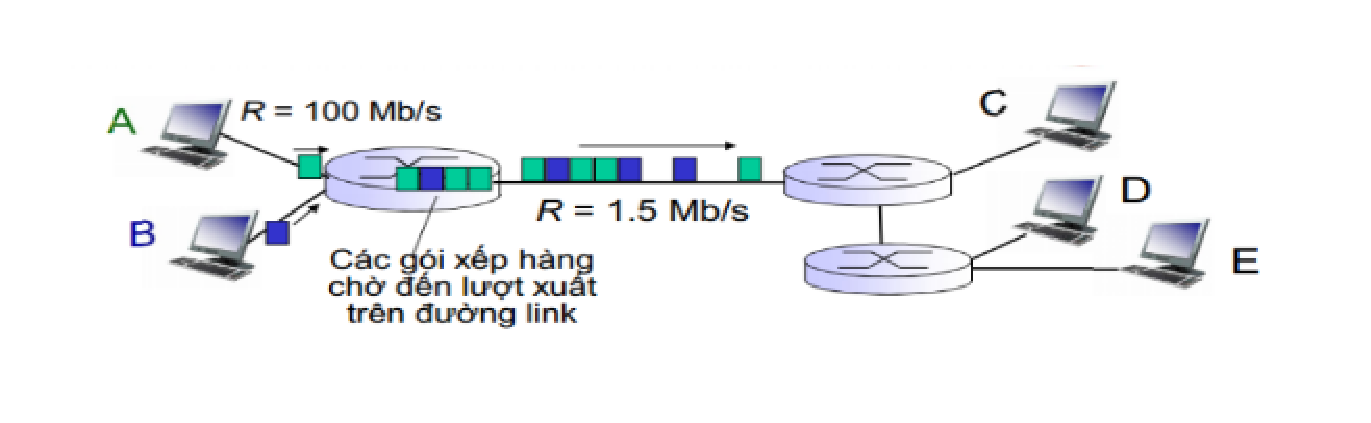
\includegraphics[scale=0.3]{q1_2}
  \end{figure}

  \item Các packet có thể bị bỏ (bị mất) nếu bộ nhớ (bộ đệm) bị đầy.
  \begin{figure}[h]
    \centering
    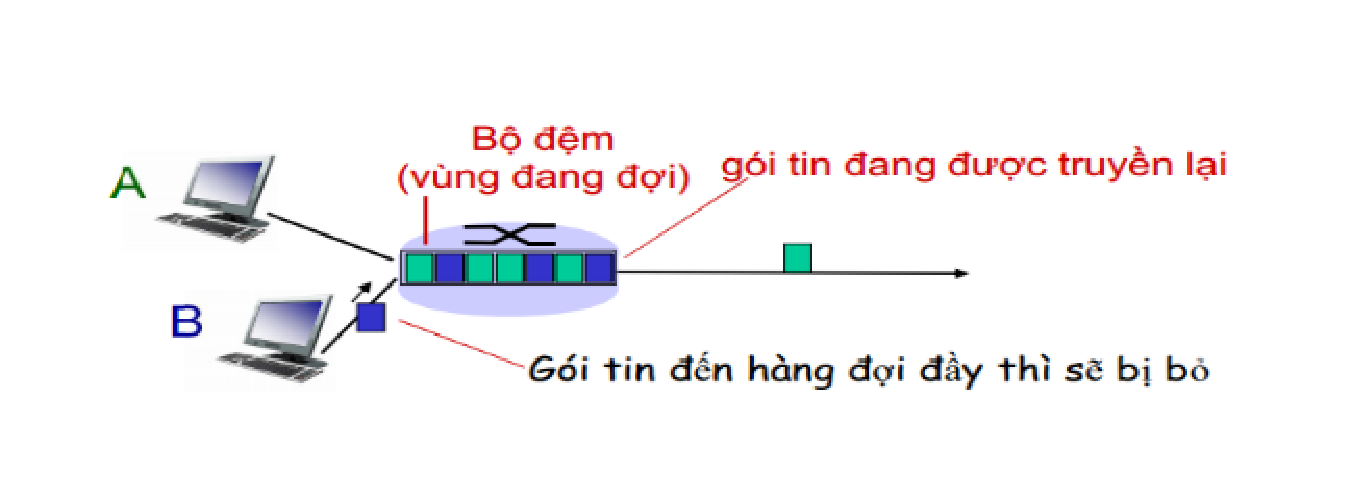
\includegraphics[scale=0.3]{q1_3}
  \end{figure}

\end{itemize}


\subsection{Chuyển mạch kênh}
Khi có hai thực thể cần trao đổi thông tin thì giữa chúng sẽ thiết lập một “kênh” (circuit) cố định 
và duy trì cho đến khi một trong hai bên ngắt liên lạc. Các dữ liệu chỉ được truyền theo con
đường cố định đó.
\begin{figure}[h]
  \centering
  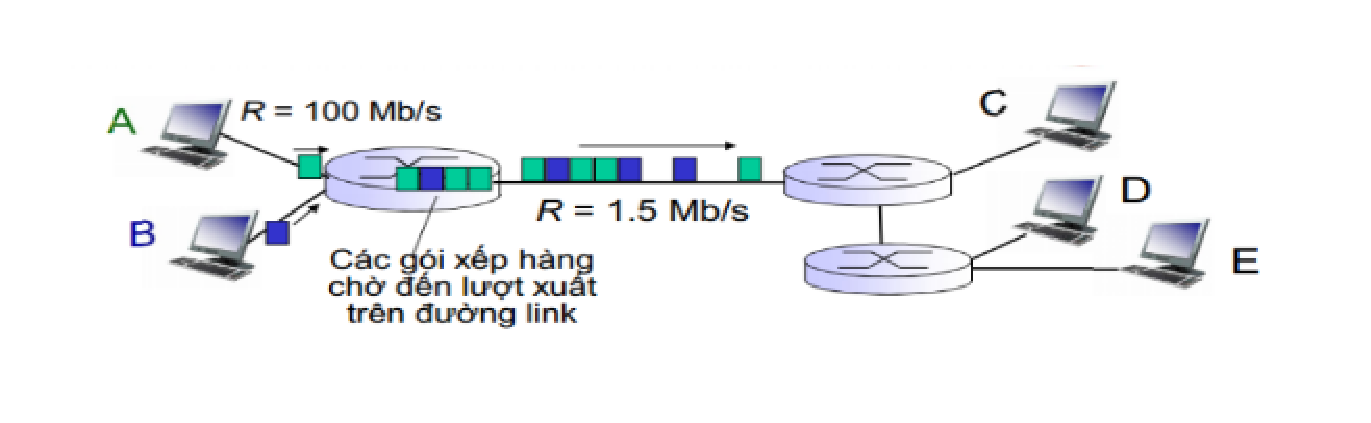
\includegraphics[scale=0.3]{q1_2}
  \caption{Chuyển mạch kênh}
\end{figure}

\subsubsection{Ưu điểm}
\begin{itemize}
  \item Dữ liệu được truyền liên tục với độ trễ rất thấp;
  \item Khó xảy ra mất dữ liệu;
\end{itemize}
\subsubsection{Khuyết điểm}
\begin{itemize}
  \item Tiêu tốn thời gian để thiết lập kênh cố định giữa hai thực thể;
  \item Hiệu suất sử dụng đường truyền không cao vì khi hai bên hết thông tin cần truyền, kênh bị bỏ không
  trong khi các thực thể khác cần không được phép sử dụng kênh;
\end{itemize}

\section{Tại sao phải phân chia mạng Internet thành nhiều tầng khác nhau ?}
Nhằm xử lý với các hệ thống phức tạp, nguyên lý “chia để trị”. Cho phép xác định rõ nhiệm vụ của mỗi bộ phận và quan hệ giữa chúng. Mô-đun hoá cho phép dễ dàng bảo trì, nâng cấp hệ thống. Thay đổi bên trong 1 bộ phận mà không ảnh hưởng tới bộ phận khác.
\begin{figure}[h]
  \centering
  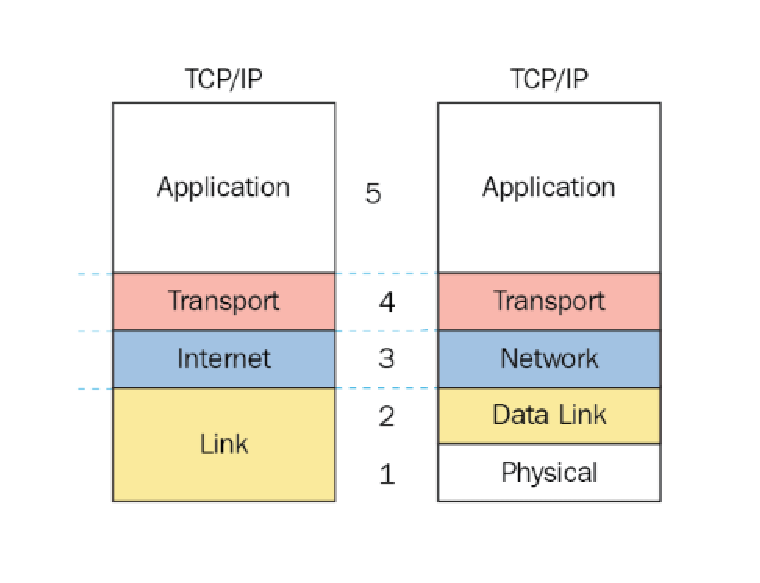
\includegraphics[scale=0.5]{q2_1}
  \caption{Một mô hình TCP/IP}
\end{figure}

Máy tính và các thiết bị kèm theo chỉ có thể hiểu và làm được những việc đã được lập trình sẵn, do đó việc phân chia theo các chức năng cụ thể là rất cần thiết. Việc gửi và nhận thông tin trên các thiết bị điện tử diễn ra theo nhiều bước và ở mỗi bước lại diễn ra những công việc khác nhau. Mô hình hay tầng mạng được phân chia dựa theo chức năng của mỗi bước khi thao tác với thông tin.


\section{Mô hình OSI}

Mô hình kết nối các hệ thống mở OSI là mô hình căn bản về các tiến trình truyền thông, thiết lập các tiêu chuẩn kiến trúc mạng ở mức Quốc tế,\;là cơ sở chung để các hệ thống khác nhau có thể liên kết và truyền thông được với nhau.

\begin{figure}[h]
  \centering
  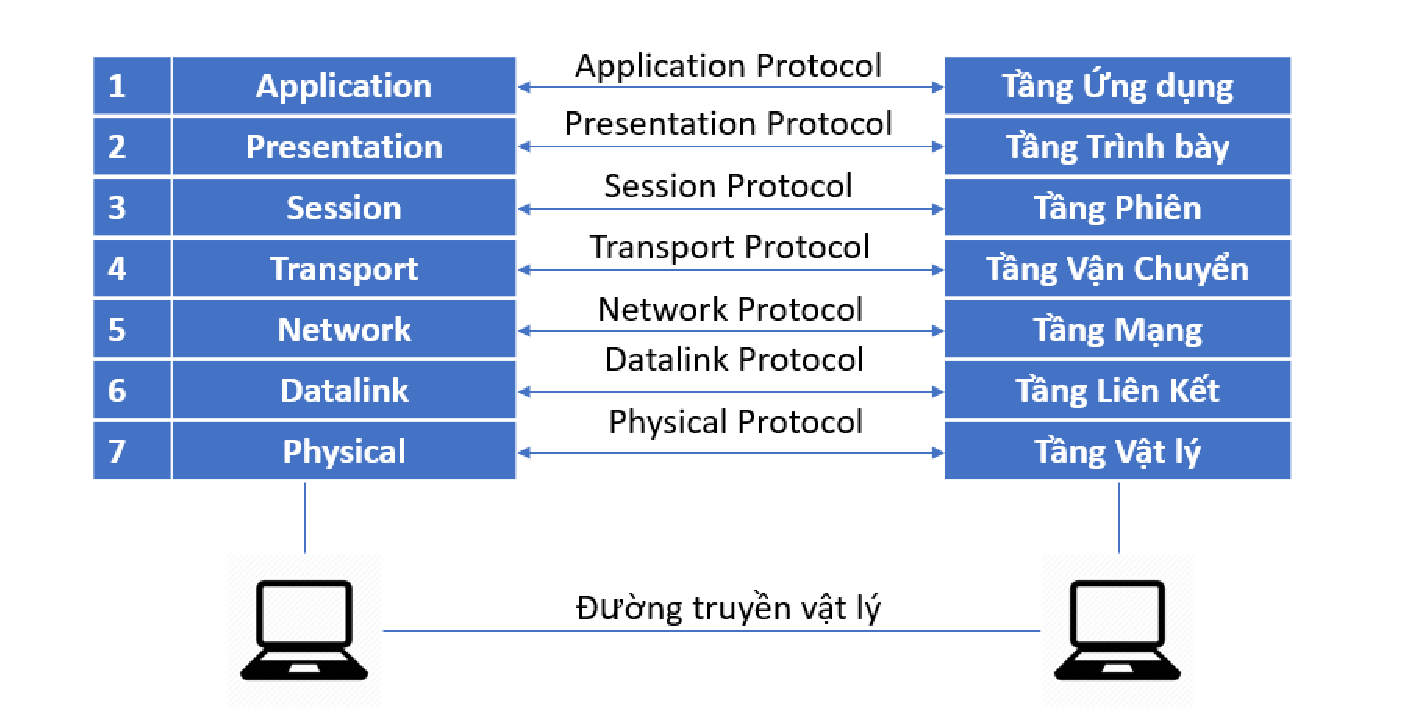
\includegraphics[scale=0.3]{q3_1}
  \caption{Một mô hình OSI}
\end{figure}

Mô hình OSI tuân theo các nguyên tắc phân tầng như sau:
\begin{itemize}
  \item Mô hình gồm 7 tầng. OSI là hệ thống mở, phải có khả năng kết nối với các hệ thống khác nhau, tương thích với các chuẩn OSI;
  \item Quá trình xử lý các ứng dụng được thực hiện trong các hệ thống mở, trong khi vẫn duy trì được các hoạt động kết nối giữa các hệ thống;
  \item Thiết lập kênh logic nhằm mục đích thực hiện việc trao đổi thông tin giữa các thực thể;
\end{itemize}
\section{Chức năng từng tầng trong mô hình OSI}
\subsection{Tầng 7: Application}
Là tầng tương tác giữa máy tính và con người, nơi ứng dụng có thể kết nối với các dịch vụ mạng. \\ \textit{VD: FTP, SMTP, HTTP}
\begin{figure}[h]
  \centering
  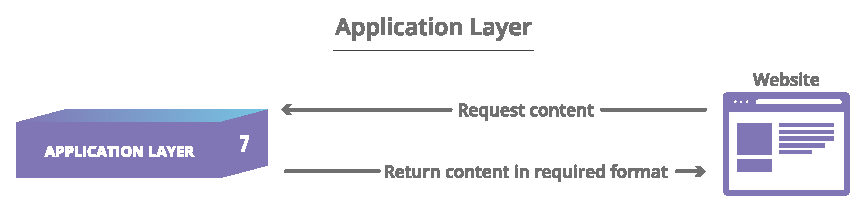
\includegraphics[scale=0.5]{q3_2}
  \caption{Tầng application của mô hình OSI}
\end{figure}

\subsection{Tầng 6: Presentation}
Đảm bảo dữ liệu ở dạng có thể sử dụng được và cũng là tầng mã hóa dữ liệu.\\ \textit{VD: ISO/IEC 8823, ISO/IEC 9576-1,  X.226, X.236}
\begin{figure}[h]
  \centering
  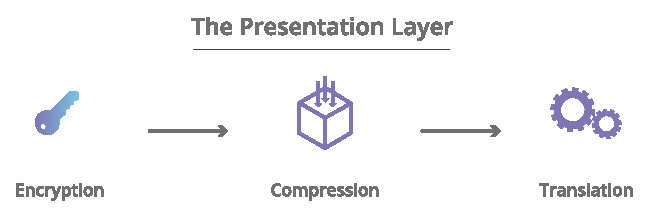
\includegraphics[scale=0.5]{q3_3}
  \caption{Tầng presentation của mô hình OSI}
\end{figure}

\subsection{Tầng 5: Session}
Duy trì kết nối và chịu trách nhiệm cho việc kiểm soát các cổng kết nối và các session.\\ \textit{VD: ISO/IEC 8327, ISO/IEC 9548-1, X.225, X.235}
\begin{figure}[H]
  \centering
  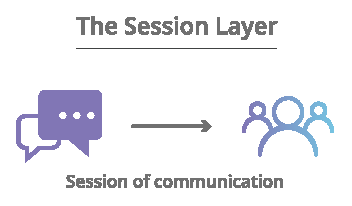
\includegraphics[scale=0.5]{q3_4}
  \caption{Tầng session của mô hình OSI}
\end{figure}

\subsection{Tầng 4: Transport}
Chuyển dữ liệu từ tiến trình này đến tiến trình kia (process-process).\\ \textit{VD: TP0, TP1, TP2, TP3, TP4}
\begin{figure}[h]
  \centering
  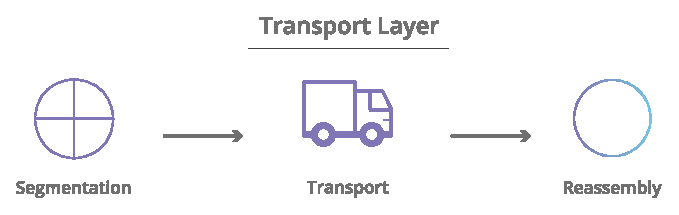
\includegraphics[scale=0.5]{q3_5}
  \caption{Tầng transport của mô hình OSI}
\end{figure}

\subsection{Tầng 3: Network}
Định tuyến những gói dữ liệu từ nguồn tới đích.\\ \textit{VD: X.225, X.223, CLNP X.233, IS-IS}
\begin{figure}[h]
  \centering
  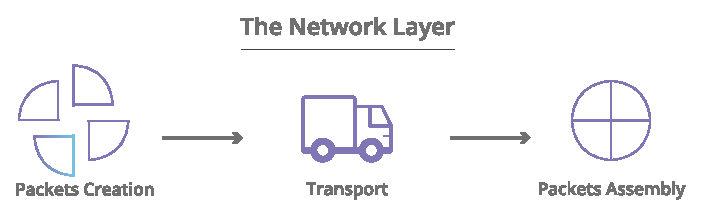
\includegraphics[scale=0.5]{q3_6}
  \caption{Tầng network của mô hình OSI}
\end{figure}

\subsection{Tầng 2: Datalink}
Chuyển dữ liệu giữa các thành phần mạng lân cận.\\ \textit{VD: X.25, Token Bus, X.222}
\begin{figure}[h]
  \centering
  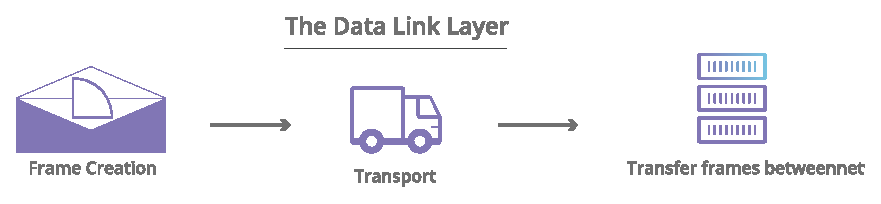
\includegraphics[scale=0.5]{q3_7}
  \caption{Tầng datalink của mô hình OSI}
\end{figure}

\subsection{Tầng 1: Physical}
Dẫn truyền luồng bit thô qua môi trường vật lý.\\ \textit{VD: X.25}
\begin{figure}[H]
  \centering
  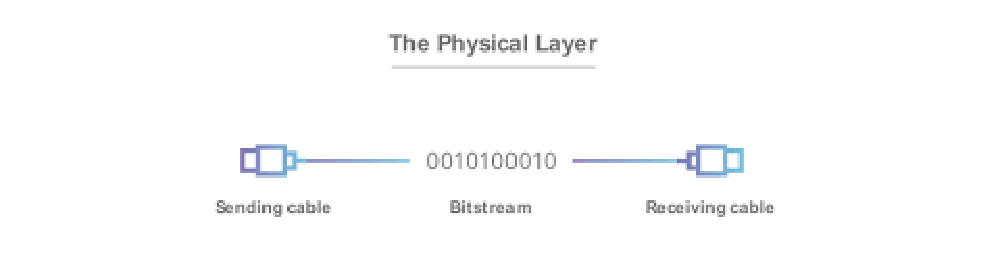
\includegraphics[scale=0.5]{q3_8}
  \caption{Tầng physical của mô hình OSI}
\end{figure}



\section{Reference}
\begin{enumerate}

  \item \href{https://www.cloudflare.com/learning/ddos/glossary/open-systems-interconnection-model-osi/}{cloudflare/open-systems-interconnection-model-osi}
  \item \href{https://en.wikipedia.org/wiki/OSI_model}{wiki/OSI-model}
  \item \href{https://imc.org.vn/tang-mang-la-gi-va-tai-sao-phai-phan-chia-tang-mang.html}{imc.org.vn}
  \item \href{https://ting3s.com/post/chuong-2-mang-may-tinh-kien-truc-phan-tang-va-mo-hinh-osi-mang-may-tinh-computer-network-309}{ting3s.com}
  \item \href{https://thanhthao94blog.wordpress.com/2015/01/14/so-sanh-chuyen-mach-goi-va-chuyen-mach-kenh/}{thanhthao94blog.wordpress.com}
\end{enumerate}

\end{document} 